\chapter{Podstawowe pojęcia}
\label{c2}

W danym rozdziale zostaną zawarte podstawowe pojęcia i mechanizmy używane przez aplikację App Inventor. Ideą tutaj jest przypomnienie oraz przypliżenie ważnych terminów informatycznych.

\section{App Inventor}
\label{c21}

W grudniu 2013 roku został wydany App Inventor w wersji drugiej. Starsza wersja została nazwana jako Classic. Oba narzędzia są bardzo podobne jednak projekty stworzone w starszej wersji nie mogą zostać zaimportowane do nowszej. W danej pracy magisterskiej skupienie zostało na nowej wersji App Inventora.

App Inventor jest to system, który pozwala na tworzenie aplikacji używając jedynie przeglądarki internetowej. Jest to aplikacja internetowa, umożliwiająca zrobienie programu, przez użytkowników mających bardzo małe pojęcie o programowaniu. 

Potencjał aplikacji jest bardzo duży. Można to zauważyć patrząc na ilość aktywnych użytkowników. W maju 2014 roku, liczba aktywnych użytkowników wynosiła 87tys. tygodniowo. Ilość zarejestrowanych to 1,9mln w 195 krajach. Użytkownicy ci stworzyli razem 4,7mln projektów.\cite{article:appinventor1}

\section{Główne komponenty}
\label{c22}

App Inventor celowo ułatwia programowanie poprzez wizualizację tworzonych komponentów i intuicyjny interfejs. App Inventor składa się z 3 głównych komponentów jakimi są:
\begin{itemize}
\item App Inventor Designer
\item App Inventor Blocks Editor
\item Android Device Emulator
\end{itemize}

\subsection{App Inventor Designer}
\label{c221}

Jednym z głównych widoków jakie można używać jest widok Designera. Projektowanie interfejsu użytkownika polega na przeciąganiu komponentów z dostępnej palety, wliczając w to także niewidoczne komponenty takie jak sensory. W tym widoku można również zmieniać właściwości obiektów, które zostały stworzone. Między innymi istnieje możliwość zmiany położenia, wielkości, układu (pionowy, poziomy).

Designer jest zaprojektowany jako zwykła aplikacja internetowa. Tak więc uruchamia się go, jak zwykłą stronę internetową wpisując jej adres www.

\begin{figure}[th] 
\centering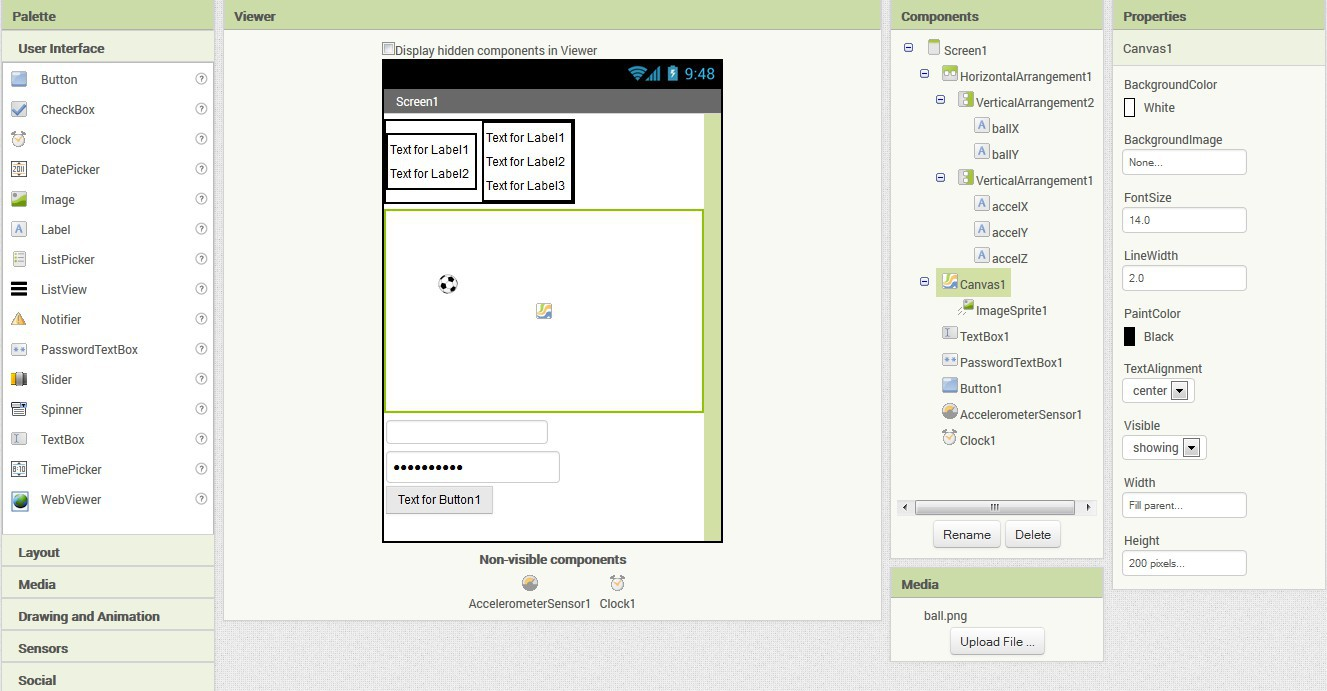
\includegraphics[width=10cm]{figures/designer}
\caption{App Inventor Designer}
\end{figure}

\subsection{App Inventor Blocks Editor}
\label{c222}

Drugim widokiem jest Blocks Editor. Zachowanie aplikacji zostaje tutaj zaprogramowane poprzez połączenie odpowiednich bloków. Istnieje możliwość korzystania z bardziej generalnych komponentów, a także z bardziej specyficznych. Dla każdego komponentu, który został stworzony w interfejsie graficznym (Designerze) są dostępne bloki mówiące, co tak naprawdę jest możliwe do zrobienia. Wygląda to w ten sposób, że komponenty są przciągane z dostępnej palety medotą "przeciągnij i upuść", a następnie łączone jak puzzle.

Ta część aplikacji normalnie reprezentowana jest przez kod napisany przez programistę. Więc napisanie zachowania aplikacji odbywa się poprzez łączenie puzzli, bez znajomości języka Java.

\begin{figure}[th] 
\centering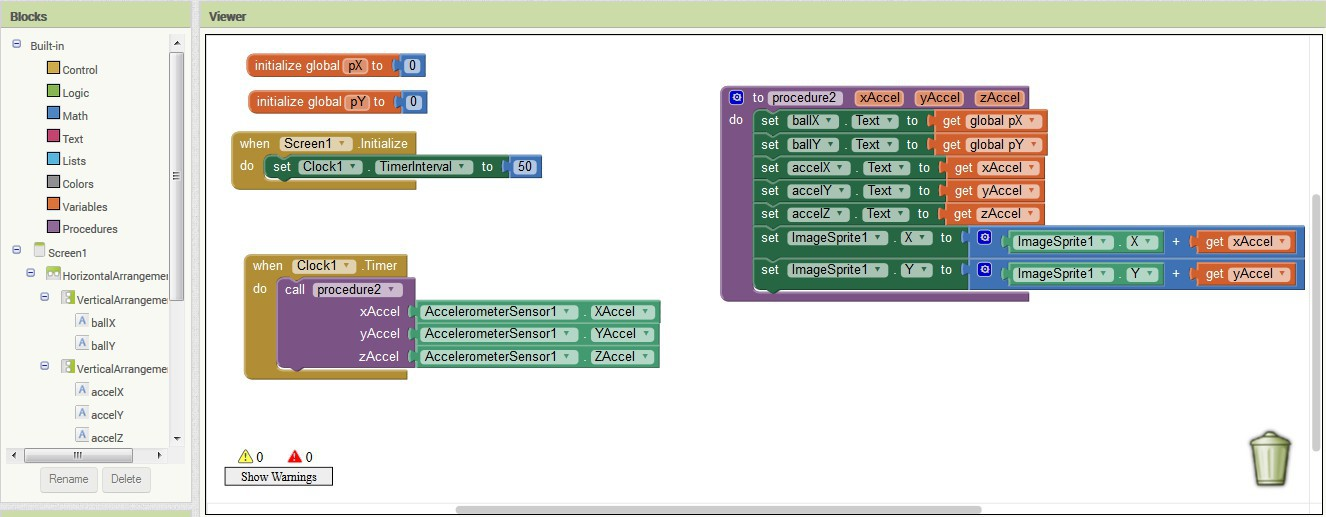
\includegraphics[width=10cm]{figures/editor}
\caption{App Inventor Blocks Editor}
\end{figure}

\subsection{Android Device Emulator}
\label{c223}

Android Device Emulator jest to emulator telefonu lub tabletu. Jest to wirtualna wersja smartphonu, w której znajdują się obsługa dotyku ekranu, przyciski systemowe oraz typowe funkcje.

Zmiany, które zostają wprowadzone, natychmiast reflektują na działanie aplikacji. Nie ma potrzeby jakiejkolwiek kompilacji i uruchamiania aplikacji od nowa. Jeżeli aplikacja zostanie uruchomiana, kompilacja zmienionych fragmentów oraz zainstalowanie ich na emulatorze dzieje się w czasie rzeczywistym. Jest to bardzo wygodna opcja budowania aplikacji i testowania jej. Zmiany, które zrobimy są od razu widoczne na ekranie.

\begin{figure}[th] 
\centering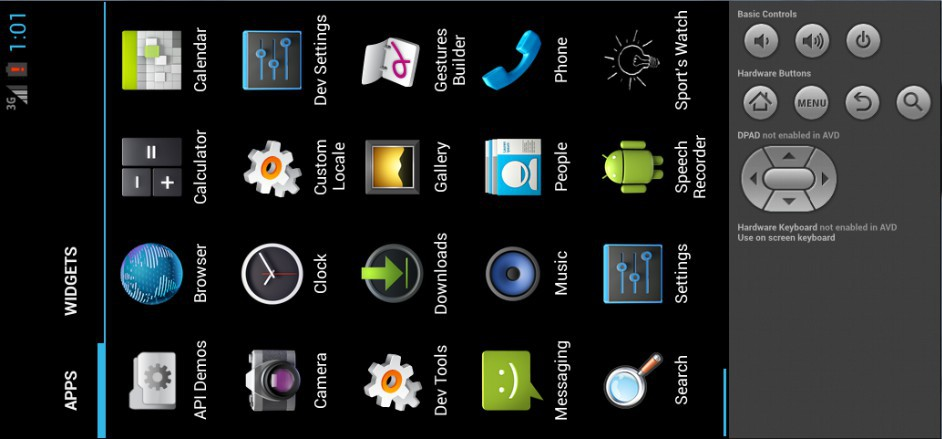
\includegraphics[width=10cm]{figures/emulator}
\caption{Android Device Emulator}
\end{figure}

\section{Pozostałe istotne komponenty}

W danym rozdziale zostały zawarte pozostałe komponenty, które zostały użyte podczas pisania pracy. Związane są one zarówno z App Inventorem, jak i z aplikacjami napisanymi w Javie.

\subsection{Android SDK}

Android SDK - jest to zestaw narzędzi programistycznych, które są oferowane dla programistów, chcących tworzyć aplikacje na platformę Android. Jest on modularny, poprzez SDK Managera, możemy zainstalować, tylko te komponenty, które nas interesują. 

\subsection{SDK Tools}

Android SDK dzieli się na dwie części SDK Tools oraz Platform Tools. Najważniejsze narzędzia wchodzące w skład pierwszej części to:
\begin{itemize}
\item AVD Manager - odpowiedzialny za zarządzanie wirtualnymi urządzeniami z systemem operacyjnym android. Jest to najłatwiejsza i najwygodniejsza opcja stworzenia nowego wirtualnego urządzenia i odpowiedniego sparametryzowania go.
\item SDK Manager - wspomniany wyżej, odpowiedzialny za instalację modułów, które nas interesują
\item Emulator - emualtor systemu android, stworzony przez AVD Managera
\item Dalvik Debug Monitor (DDMS) \label{ddms}- jest to narzędzie pomocne w debugowaniu aplikacji. Dostarcza on takich funkcji jak przekierowanie portów, przechwyt obrazu na urządzeniu, informacje o wątkach, stosie, a także o metodach, które są uruchomione jeżeli włączymy ich profilowanie.
\end{itemize}

\subsection{Platform Tools}

\begin{itemize}
\item Android Debug Bridge \label{adb}- narzędzie pozwalające na komunikację z podłączonym urządzeniem. Jest także używany do instalacji i uruchamiania aplikacji. Składa się z 2 części, klienta i serwera, które komunikują się ze sobą.
\end{itemize}

\subsection{Apktool}

Jest to narzędzie do tak zwanej inżynierii odwrotnej (\english{Reverse engineering}). Umożliwia ono dekodowanie programu do prawie oryginalnej formy. Następnie, po dokonaniu pewnych modyfikacji umożliwia ono zbudowanie aplikacji z powrotem do wyjściowej formy.\cite{doc:apktool}

\subsection{Keystore}

Jest to repozytorium przechowujące certyfikaty bezpieczeństwa. Do zarządzania certyfikatami istnieje narzędzie o nazwie keytool. Umożliwia ono użytkownikom zarządzanie prywatnymi/publicznymi kluczami, certyfikatami jak i podpisem elektornicznym.\cite{doc:keytool}

\subsection{Jarsigner}

System android wymaga, aby aplikacje na nim instalowane były cyfrowo podpisane. Dzięki temu system może zweryfikować autora aplikacji. Podpisywanie aplikacji dzielimy na 2 sposoby: tryb debugowania (\english{Debug mode})oraz tryb wydania (\english{Release mode}). Przy korzystaniu ze zintegrowanego środowiska programistycznego zwykle aplikacja zostaje cyfrowo podpisana automatycznie, podczas instalacji jej na telefonie. Jarsigner umożliwia popisanie aplikacji manualnie, korzystając z lini poleceń.

\subsection{Zużycie procesora}

Czas pracy procesora jest to czas, w którym procesor (\english{CPU}) został użyty to przetwarzania zadanych instrukcji, w przeciwieństwie do oczekiwania na wejście/wyjście lub przejścia w stan oczekiwania (\english{Idle mode}). Zużycie procesora natomiast mierzone jest w procentach jako całkowitej wydajności procesora. Główne zastosowanie to określenie ogólnej zajętości systemu. Wysokie zużycie procesora oznacza zbyt małą moc procesora, lub zbyt wygórowane oczekiwania użytkownika.


\section{Ważne koncepcje i pojęcia dotyczące App Inventora}

Istnieje kilka pojęć, które są warte uwagi. Zostały one zawarte w tym rozdziale.

\subsection{Publikacja aplikacji na Google Play}

Aplikacje zbudowane za pomocą App Inventora mogą zostać przesłane do marketu Google Play. Każda aplikacja, która ma zostać opublikowana musi posiadać wersję kodu (\english{VersionCode}) oraz nazwę wersji (\english{VersionName}). Te parametry można ustawić we właściwościach głównego komponentu\cite{doc:concepts}. Wersja kodu jest to całkowita wartość, która nie jest widoczna dla użytkowników w Google Play. Potrzebna jest do sprawdzenia czy aplikacja została aktualizowana lub dezaktualizowana do poprzedniej wersji. Nazwa wersji może być dowolna jednak wg konwencji powinna to być liczba zmiennoprzecinkowa. Domyślnie posiada wartość 1.0. Jest ona zwiększana o 0.1 lub 1 dla małej i dużej zmiany.

Skończony projekt możemy wyeksportować do pliku .apk, który jest automatycznie cyfrowo podpisany kluczem prywatnym powiązanym z naszym kontem. Kiedy tworzymy nową wersję ten sam klucz jest używany do podpisu. Kiedy urządzenie z system android posiada zainstalowaną aplikację, zapamiętuje on klucz który został użyty do podpisu. Aby zainstalować wyższą wersję aplikacji ten sam klucz musi zostać użyty do podpisu.

Repozytorium keystore, w którym znajduje się klucz domyślnie jest stworzone na serwerze, więc nie trzeba się tym martwić. Istnieje również opcja eksportu i importu repozytorium. Jest ona przydatna przy przenoszeniu projektu na inny serwer.

\subsection{Paleta z dostępnymi komponentami}

\begin{itemize}

\item \textbf{User Interface} - w większości widoczne komponenty, które są związane z interfejsem użytkownika.
\begin{itemize}
\item Button - przycisk.
\item CheckBox - pole wyboru.
\item DatePicker - komponent dający możliwość wyboru daty.
\item Image - komponent umożliwiający wyświetlenie przesłanego zdjęcia.
\item Label - etykieta, na której zwykle wyświetlany jest kawałek tekstu.
\item ListPicker - komponent, który po kliknięciu wyświetla listę, z której użytkownik może wybrać wartość. Daje on także możliwość automatycznego osadzenia wyszukiwarki na liście.
\item ListView - komponent, który pozwala na osadzenie i wyświetlenie listy elemenentów
\item Notifier - komponent wyświetlający powiadomienia, a także umożliwiający logowanie na 3 poziomach (Error, Warn, Info).
\item TextBox - komponent umożliwiający wpisywanie tekstu.
\item PasswordTextBox - taki sam komponent jak TextBox jednak wpisywany tekst nie jest widoczny dla użytkownika.
\item Slider - jest to pasek postępu, który dodatkowo umożliwia użytkownikowi przeciąganie.
\item Spinner - element wyświetlający pop-up z listą elementów do wyboru.
\item TimePicker - element pozwalający na wybór czasu.
\item WebViewer - komponenet umożliwiający umieszczenie dowolnej strony internetowej w aplikaji.
\end{itemize}

\item \textbf{Layout} - Komponenty odpowiedzialne za rozmieszczenie pozostałych komponentów. Są to kontenery, w które mogą zostać umieszczane inne widoczne komponenty.
\begin{itemize}
\item HorizontalArrangement - elementy umieszczone w tym kontenerze są układanej od lewej do prawej.
\item VerticalArrangement - odwrotne działanie do poprzedniego komponentu - elementu są umieszczany od góry do dołu.
\item TableArrangement - element umożliwiający ustawienie elementów postaci tabularnej
\end{itemize}


\item \textbf{Media} - Komponenty związane głównie z dźwiękiem oraz kamerą.
\begin{itemize}
\item Camcorder - komponent umożliwiający nagrywanie filmów. Istnieje możliwość nadania nazwy pliku zawierającego nagranie.
\item Camera - komponent umożliwiający robienie zdjęć i zapisywanie ich.
\item ImagePicker - komponent uruchamiający galerię zdjęć zawartą na telefonie i dający możliwość wyboru zdjęciu. Zdjęcie po wybraniu jest kopiowane na kartę SD (maksymalna ilość zdjęć to 10). Następnie możemy z danego zdjęcia skorzystać w aplikacji i je wyświetlić.
\item Player - komponent odtwarząjący muzykę, a także odpowiedzialny za wywołanie wibracji w telefonie.
\item Sound - komponent odtwarzający dźwięki, w porównaniu do poprzedniego, dźwięki powinny mieć krótki czas trwania, podczas gdy muzyka może trwać długo.
\item SoundRecorder - komponent nagrywający dźwięk
\item SpeechRecognizer - komponent umożliwiający rozpoznanie mowy i stworzenie z niej tekstu
\item TextToSpeech - komponent o odwrotnym działaniu do poprzedniego, zamieniający tekst na mowę. Wsparcie dla języków: czeski, hiszpański, niemiecki, francuski, duński, włoski, polski, angielski.
\item VideoPlayer - komponent umożliwiający odtwarzanie filmu podczas działającej aplikacji. Pliki wideo muszą mieć poniżej 1MB, dodatkowo rozmiar całkowitej aplikacji wynosi maksymalnie 5MB.
\item YandexTranslate - komponent umożliwiający tłumaczenie tekstu pomiędzy językami. Korzysta on z serwisu o nazwie Yandex - https://translate.yandex.com. dodatkowo urządzenie musi być podłączone do internetu. 
\end{itemize}


\item \textbf{Drawing and Animation} Komponenty umożliwiające rysowanie oraz animacje.
\begin{itemize}
\item Canvas - płótno, na którym możemy rysować dwuwymiarowe obrazki (\english{Sprite}). Obrazki te mogą się na płótnie poruszać. Każda lokalizacja na płótnie jest specyfikowana za pomocą współrzędnych X,Y.
\item ImageSprite - obrazek, który możemy umieścić na płótnie i który może reagować na dotyk, przeciąganie
\item Ball - jest to ImageSprite, który ma ustawiony obrazek jako koło o określanym kolorze.
\end{itemize}

\item \textbf{Sensors} Niektóre z sensorów, dostępnych na telefonie. Wszystkie z tych komponentów są niewidoczne.
\begin{itemize}
\item AccelerometerSenser - akcelerometr, komponent, który umożliwia wykrycie trzęsienia telefonem, a daje wartości, odpowiadające aktualnemu wychyleniu telefonu.
\item BarcodeScanner - komponent umożliwiający skanowanie kodów kreskowych, jednak musimy posiadać dodatkowo aplikację do tego zainstalowaną już na telefonie.
\item Clock - Zegar oraz czasomierz
\item LocationSensor - komponent dostarczający informacje o położeniu gdzie się znajdujemy, czyli szerokość i długość geograficzną. Informacje te mogą nie być odrazu dostępne i musimy na nie poczekać.
\item NearField - komponent dostarczający możliwośći NFC. Dotychczas komponent ten umożliwia czytanie i wysyłanie tagów tekstowych.
\item OrientationSensor - żyroskop - komponent dostarczający informację o urządzeniu w 3 wymiarach.
\end{itemize}

\item \textbf{Social} - komponenty związane z kontaktami, e-mailami i serwisami społecznościowymi.
\begin{itemize}
\item ContactPicker - przycisk, który po naciśnięciu wyświetla listę kontaktów do wyboru. Gdy użytkownik dokona wyboru ma dostęp do następujących danych: nazwa kontaktu, e-maile, telefony, zdjęcie kontaktu.
\item EmailPicker - textBox z pomocą dla użytkownika. Pomoc ta polega na wyświetleniu listy, która zawiera emaile pasujące do wpisywanego tekstu.
\item PhoneCall - komponent umożliwiający uruchomienie dzownienia do osoby, którą wcześniej ustawimy jako właściwość komponentu.
\item PhoneNumberPicker - przycisk o podobnym działaniu do komponentu ContactPicker.
\item Sharing - niewidoczny komponent, który umożliwia udostępnienie wiadomości lub pliku innym aplikacjom
\item Texting - komponent odpowiedzialny za zarządzanie wiadomościami. Jeżeli aplikacja działa w tle, zdarzenie przyjścia wiadomości również będzie uruchomione. Nawet jeżeli aplikacja nie jest uruchomiona pojawi się powiadomienie o przyjściu wiadomości, po kliknięciu w nie uruchomi się aplikacja
\item Twitter - komponent umożliwiający komunikację z serwisem internetowym Twitter. Jeżeli użytkownik zostanie pozytywnie zautentykowany i zautoryzowany, pojawia się wiele możliwości, min. szukanie tweetów, wysyłanie tweetów, wiadomości, obrazków.
\end{itemize}

\item \textbf{Storage} - komponenty odpowiedzialne za przechowywanie danych.
\begin{itemize}
\item File - niewidoczny komponent umożliwiający zapis i odczyt pliku. Domyślne ustawienia zapisują pliki do prywatnego katalogu App Inventora, jednak istnieje możliwość ustawienia innej ścieżki
\item FusiontablesControl - komponent, który komunikuje się z serwisem internetowym dostarczonym przez Google o nazwie Fusion Tables. Tabele te umożliwiają wizualizację, udostępnienie, zapis danych. Komponent ten daj możliwość dostępu do tych danych a także jej edycji.
\item TinyDB - baza danych dla aplikacji. Jest to odpowiednik klasy Javy - SharedPreferences. Można sobie ją wyobrazić jako mapę - klucz/wartość.
\item TinyWebDB - niewidoczny komponent, komunikujący się z internetową bazą danych.
\end{itemize}

\item \textbf{Connectivity} - komponenty umożliwiające komunikację i uruchmianie innych apliakcji.
\begin{itemize}
\item ActivityStarter - komponent do uruchamiania zewnętrznych Activity. Przez Activiy są rozumiane: inne aplikacji napisane w App Inventorze, kamera, wyszukiwarka internetowa, otwieranie strony internetowej, otwieranie aplikacji mapy w zadanej lokalizacji.
\item BluetoothClient - komponent blutetooth klienta.
\item BluetoothServer - komponent bluetooth serwera.
\item Web - komponenet umożliwiający wysyłanie żądań typu REST do serwera. Dostarcza od funkcje: GET, POST, PUT, DELETE.
\end{itemize}

\item \textbf{LEGO MINDSTORMS} - komponenty dostarczające kontrolę nad robotami poprzez bluetooth. W danej pracy magisterskiej zostały pominięte, ze względu na brak powyższych robotów.
\end{itemize}

\subsection{Dostępne bloki}

\begin{itemize}

\item Control - bloki odpowiedzialne za przepływ w aplikacji. Znajdują się tutaj instrukcje warunkowe if-else, pętle for, foreach, while, do-while. Inne bloki w tej sekcji są odpowiedzialne za otwieranie innych aplikacji lub zamykanie aktualnej.

\item Logic - bloki odpowiadające za logikę. Kiedy istnieje potrzeba stworzenia instrukcji warunkowej zazwyczaj korzysta się z tych bloków. Sprawdzają one czy zmienne są takie same lub różne. Są tutaj też wartości true i false.

\item Math - bloki odpowiedzialne za wyrażenia matematyczne, min. takie jak dodawanie, odejmowanie, mnożenie, dzielenie. Ale są tu również funkcji pomocniczne, np. konwersja radianów do stopni lub odwrotnie, funkcje trygonometryczne, minimum dla zadanych argumentów, losowa wartość.

\item Test - bloki odpowiedzialne za zarządzanie tekstem. Jest tutaj większość funkcji znanej klasy String z Javy. Sprawdzenie czy zmienna jest pusta, ilość znaków, zamiana występnień danego elementu.

\item Lists - bloki tworzące listy oraz zarządzające nimi. Istnieje możliwość dodawania, usuwania, zamiany elementów na liście za pomocą oferowanych funkcji. Dodatkowe funkcji znajdujące się tutaj to funkcje konwertujące listę do formatu wiersza lub tabeli, który można następnie umieścić w pliku csv.

\item Colors - bloki z kolorami, które można przypisać stworzonym komponentom. Istnieje także możliwość zdefiniowania własnego koloru.

\item Variables - bloki odpowiedzialne za tworznienie zmiennych lokalnych i globalnych. Znajdują się tutaj też bloki inicjalizujące i odczytujące wartość zmiennych (\english{settery i gettery}).

\item Procedures - bloki tworzące procedury oraz funkcje zwracające wartość.

\end{itemize}

\subsection{Android - przechowywanie danych}

Urządzenie z systemem android dostarcza szereg mechanizmów dotyczących przechowywania danych. Każdy z nich stosujemy do czegoś innego.

\begin{itemize}
\item SharedPreferences - przechowuje pary klucz-wartość, czyli niewielkie ilości danych. Mechanizm wykorzystywany jest przede wszystkim do przechowywania ustawień aplikacji.\cite{tutorial:sqlite}
\item Baza danych SQLite – wykorzystywane do przechowywania dużej ilości uporządkowanych danych, które ze względu na swoja ilość wymagają wysokiej wydajności dostępu.\cite{tutorial:sqlite}
\item Pliki - w związku z wykorzystaniem bazy SQLite, która nie obsługuje przechowywania plików, dane binarne (zdjęcia, filmy, inne pliki) powinniśmy przechowywać w ich niezmiennej formie, na karcie lub pamięci wbudowanej w urządzenie.\cite{tutorial:sqlite}
\end{itemize}









